\chapter{InMourning Prototype}

\section{Background: Bereavement Technologies}
  For inspiration and guidance for this initial prototype,
  I looked into existing bereavement technologies.
  Research into bereavement from the perspective of HCI is young, but the
  existing literature reveals some of the core problems that technology can
  address. Among the earliest research is that of Massimi and Baecker in 2010
  \cite{mm10},
  a needs-analysis of all the ways that technology intersects with the lives of
  the bereaved.
  Part of their study was an observation of how,
  in the potentially-dispersed setting of the modern world, 
  technology is already used to help bring people together during mourning.
  Massimi and Baecker proposed a wide set of design opportunities and challenges.
  They were primarily interested in exploring technological artifacts,
  both inherited from the deceased and those created by the bereaved to
  remember and grieve, but they also mention the possibility of technology
  helping to provide social support.

  % Homescreen Figure
  \begin{figure}
  \caption{\textbf{Besupp Screenshot} --
  Besupp offered circles for people with like losses to share thoughts
  and feelings with each other.
  }
  \centering
  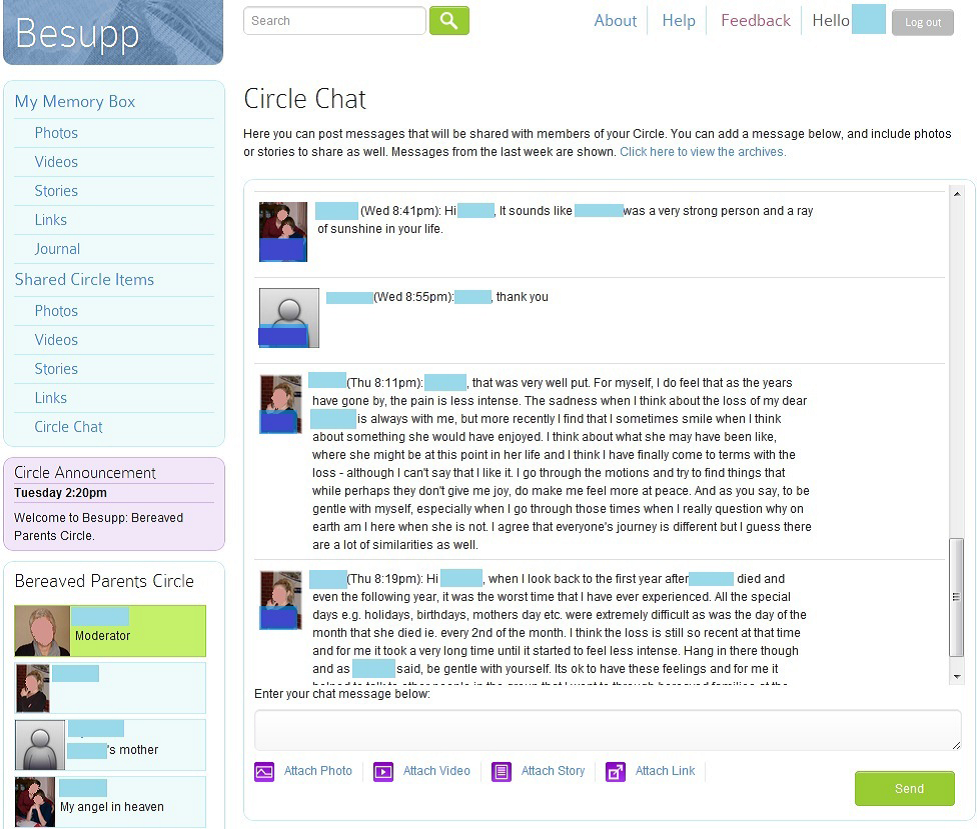
\includegraphics[width=0.65\textwidth]{besupp.png}
  \label{fig:besupp}
  \end{figure}

  There have been few technologies designed explicitly for the grieving. One
  example is Besupp, an online platform for maintaining a support group between
  people who have experienced similar losses, designed and tested by Massimi and
  co. in 2013. \cite{mm13}
  A screenshot from the study is shown in Figure \ref{fig:besupp}.
  Massimi and co. observed that technologies can be helpful as
  one of many ways to help with coping, as the needs of the bereaved are best
  addressed by a variety of interactions.
  This further study demonstrated that
  there is value in support systems that are maintained over long periods and
  designed for to low and intermittent usage.

  Other research has generally been observational, for instance Brubaker's study
  in 2011 of usage of existing technologies. \cite{brubaker11}

\section{TBD}
Import all the proposal materials!

\section{Maturation into InMind}
  However, we soon ran into a problem.
  If we want to use technology to improve the relationships between friends and family during the
  process of bereavement, we have to introduce technology well before the crisis happens.
  This is for primarily two reasons.
  \begin{enumerate}
  \item Death is often a stunning, overwhelming catastrophe,
  and bereaved individuals cannot be burdened with learning how to use a new technology.
  Many recently bereaved individuals already find it difficult to do things they normally can. \cite{??}
  \item For the deaths that are more forseeable, such as due to illness,
  there is often a long period of handling the dire situation,
  in which many of the same needs exist.
  In fact, mourning can sometimes begin before the death. \cite{??}
  \end{enumerate}

\clearpage
\newpage
